\section{Appendix}

In this section, we delve into the implementation of the innovative algorithms that power DefiPlaza on Radix. The fundamental price algorithm adheres to the definitions and notations established by Dodo. Tokens are consistently traded in pairs, with $B$ denoting the 'base' token and $Q$ signifying the 'quote' token. The spot price, represented by $p$, corresponds to the number of quote tokens offered by the algorithm for each base token. The spot price is adjusted for trade size (\textit{price impact}). At equilibrium, the quantity of base tokens ($B_0$) is equivalent to the sum of the added liquidity and accumulated fees. Likewise, the number of quote tokens reaches equilibrium at $Q_0$. The reference price, denoted as $p_0$, represents the market price at which the exchange achieves equilibrium.

\subsection{Price function}
After a user executes a trade against the liquidity in the pool, the token holdings deviate from their equilibrium values. To encourage users to trade back towards equilibrium the Dodo algorithm adjusts the spot price as per equation \ref{eq:priceCurve}.

\begin{align} \label{eq:priceCurve}
	p &= p_0 \left( 1 + k \frac{B_0^2 - B^2}{B^2} \right)
\end{align}

The liquidity concentration factor, denoted as $k$, can range from $0$ (representing a constant sum exchange) to $1$ (indicating a constant product exchange). As the value approaches zero, the liquidity concentration around the reference price intensifies. It is important to note that theoretically, there is no constraint on using values above one; however, this would result in a more rapid increase in price as reserves change. In other words, employing a value greater than $1$ implies that the exchange offers liquidity surpassing that of the constant product exchange. It should be noted that equation \ref{eq:priceCurve} presumes a deficiency of base tokens in the pool (i.e., $B < B_0$). Conversely, in situations where there is a shortage of quote tokens, the price adheres to equation \ref{eq:priceQuote}.

\begin{align} \label{eq:priceQuote}
	p &= \frac{p_0}{ 1 + k \frac{Q_0^2 - Q^2}{Q^2}}
\end{align}

For convenience, the rest of the text it is assumed that the exchange has a shortage of base tokens. All of the calculations can easily be converted to the symmetric case of quote shortage where needed.

\subsection{Swap curves}
When a trade takes place during a shortage of base tokens, the price offered follows equation \ref{eq:priceCurve} along the curve. The amount of tokens offered can be calculated by integrating equation \ref{eq:priceCurve} over the the $B$ tokens traded. Equation \ref{eq:swapIn} describes the curve between the amount of quote tokens taken in against the amount of base tokens taken from (and remaining in) the pool.

\begin{align} \label{eq:swapIn}
	\Delta Q  &= \frac{\Delta B \left(B + k \Delta B \right)}{B} p_0
\end{align}

Equation \ref{eq:priceQuote} uses delta values for $B$ and $Q$ with respect to their reference values $B_0$ and $Q0$. The equation can be used directly the algorithm to compute the amount of quote tokens to return when swapping back towards equilibrium. We can record the $Delta Q$ before the trade, adjust $B$ and $\Delta B$ for the amount of incoming tokens and calculate the new value for $\Delta Q$. Although equation \ref{eq:swapIn} can be used for trades returning to equilibrium, it needs to be rewritten for a trade in the other direction. Equation \ref{eq:swapOut} gives the value for $\Delta B$ for a given value of $\Delta Q$.

\begin{align} \label{eq:swapOut}
	\Delta B &= \frac{B_0 + \frac{\Delta Q}{p_0}}{2\left(1-k\right)} - \frac{\sqrt{B_0^2 + \left(4k-2\right)B_0 \frac{\Delta Q}{p_0} + \left(\frac{\Delta Q}{p_0}\right)^2}}{2\left(1-k\right)}
\end{align}

It can be observed that equation \ref{eq:swapOut} encounters a breakdown when the liquidity concentration factor $k$ equals $1$, as this causes the denominators to reach zero. The constant product case, represented by a $k$ value of $1$, constitutes a unique scenario for which equation \ref{eq:swapOut} can be reduced to the more streamlined form expressed in equation \ref{eq:swapOutSpecial}.

\begin{align} \label{eq:swapOutSpecial}
  \Delta B = \frac{B_0 \Delta Q}{B_0 p_0 + \Delta Q}
\end{align}

Thus far, we have not addressed the appropriate value for the liquidity concentration factor $k$. The innovative methodology employed by DefiPlaza on Radix involves modulating the degree of concentration $k$ when executing trades that deviate from equilibrium (as illustrated in equation \ref{eq:swapOut}), in contrast to the concentration when trading converges back toward equilibrium, as depicted by equation \ref{eq:swapIn}.

To elaborate, we designate $k_{in}$ as the liquidity concentration factor employed when trading returns to equilibrium, and $k_{out}$ as the factor utilized when trading deviates from equilibrium. By establishing $k_{out} > k_{in}$, we effectively provide more limited liquidity when diverging from equilibrium compared to when trading converges back toward equilibrium. Taking $k_{in}$ as the reference curve, we can deduce that upon completion of a trade away from equilibrium using $k_{out}$, an excess of quote tokens remains in the pool relative to the number of base tokens withdrawn. This surplus of quote tokens can be strategically employed to adjust the reference price $p_0$ in the direction of the market price, without imposing a loss on liquidity providers.

We assume that normally we are operating on the curve with the higher $k$ value. This curve fixes the relationship between $p_0$, $\Delta B$ and $\Delta Q$. If we then decide to trade on another $k$ value for trades away from equilibrium, we need to use virtual values to ensure the spot price is the same at the current operating point. Using the prime notation to indicate virtual values we can calculate $p_0'$ and $\Delta Q'$ as given below:

\begin{align} \label{eq:PZeroPrime}
  p_0' &= \frac{B^2 + k_{in} \left( B_0^2 - B^2 \right)}{B^2 + k_{out} \left( B_0^2 -B^2 \right)} p_0 \\
  \Delta Q' &= \frac{\Delta B \left(B + k_{out} \Delta B \right)}{B} p_0'
\end{align}

Trades away from equilibrium are executed against the virtual reference price and the virtual $\Delta Q$ reserves as above, while trades towards equilibrium are executed against the real values for reference price and $\Delta Q$.

When a trade away from equilibrium has been completed, the pair now holds more $\Delta Q$ than it would have for the same change in $\Delta B$ under the reference curve for $k_{in}$. When taking a trade in the other direction, the reference curve needs to be shifted to account for the additional tokens. This shift is realized by updating the reference price $p_0$ which now functions as an internal oracle that slowly tracks the market price. Equation \ref{eq:p0Shift} is used to calculate the new value for $p_0$.

\begin{align} \label{eq:p0Shift}
  p_0 &= \frac{B \Delta Q}{\Delta B \left( B + k_{in} \Delta B \right)}
\end{align}

Note that $k{in}$ and $k_{out}$ are design parameters. They represent the amount of concentration on trades towards equilibrium vs trades away from equilibrium. The ratio between the two determines to what extent the liquidity offered differs. A higher ration means more aggressive updating of the internal oracle at the cost of lower expected trade volume. The swap process is depicted as a flowchart in figure \ref{fig:flowchart}.

\begin{figure} 
  \centering
    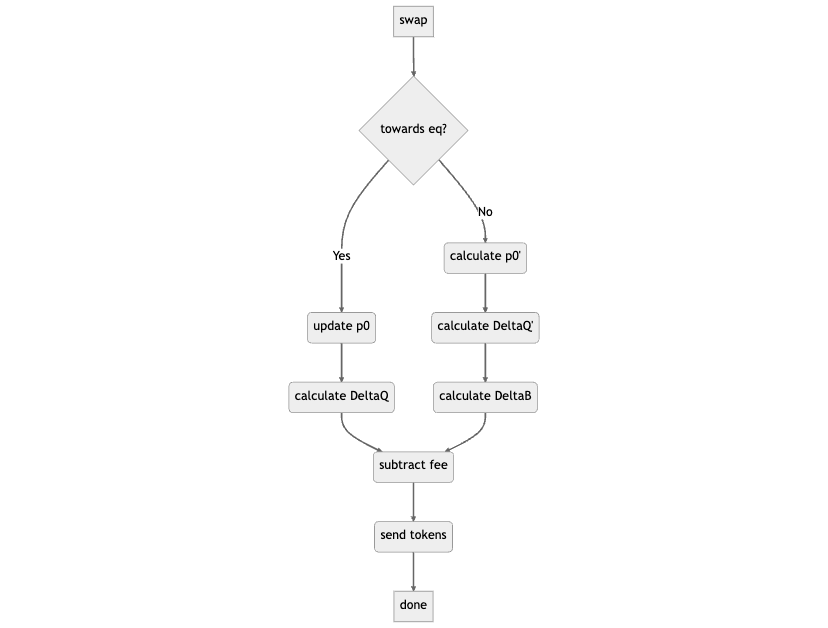
\includegraphics[scale=0.5]{flowchart.png} 
    \caption{Swap function flowchart}
      \label{fig:flowchart}
\end{figure}


\subsection{Liquidity Add}

\subsection{Liquidity Remove}
Removing liquidity from a token within a pair is comparatively simple. There are two cases:
\begin{itemize}
	\item Token is not in shortage: If the token that is withdrawn from the exchange is not in shortage, we can simply calculate the fraction of tokens that corresponds to a given amount of LP tokens. Removing the liquidity is simply withdrawing this fraction and burning the LP tokens.
	\item  
\end{itemize}